\section{Arquitectura de la Solución}

La figura X muestra un diagrama de arquitectura de la solución, para
soportar los procesos de análisis y extracción de datos, así como la
visualización de los mismos.
La participación de cada uno de los componentes de la solución en las distintas
etapas, será explicado en las próximas secciones.

\begin{figure}[H]
    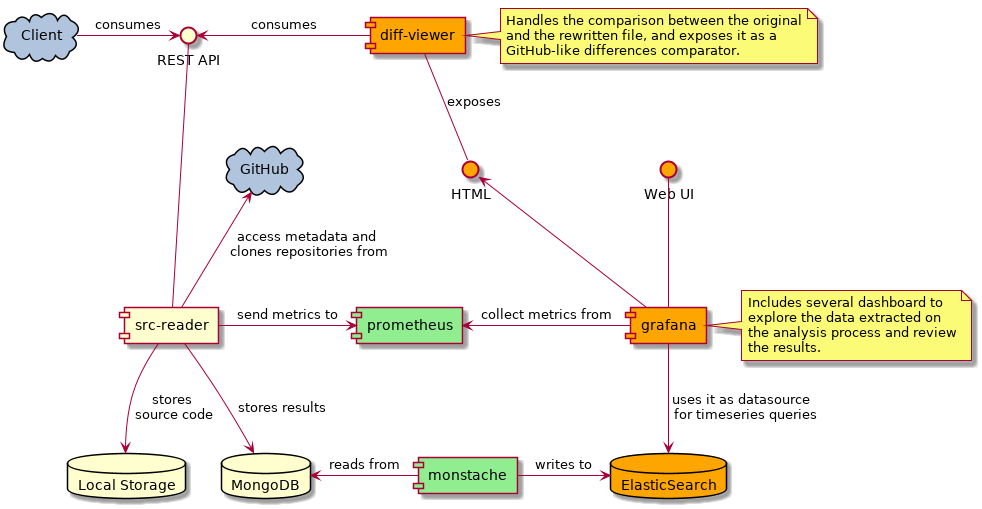
\includegraphics[width=12cm]{implementation/architecture_overview.png}
    \centering
    \caption{Arquitectura general de la Solución}
  \end{figure}

\subsection{Fase: Cálculo}

Tal como se enunció anteriormente, la fase de cálculo consta de diferentes etapas,
cada una con un objetivo bien claro.
Estas etapas se suceden unas a otras, utilizando la salida de una estapa previamente
ejecutada, como entrada para la siguiente, presentando así una cierta secuencialidad.

%extracción, procesamiento y cálculo.

\subsubsection{Etapa: Extracción}

Para poder dividir y expandir los identificadores que forman parte de una base de código de fuente, 
primero necesitamos analizar los archivos que lo componen y construir los árboles de sintáxisis
abstracta, que serán procesados en la etapa siguiente.
Los pasos que forman parte 
Este proceso, definido como \textbf{extracción}, y contiene diferentes pasos,
dentro de los que encontramos:

\begin{enumerate}
  \item Clonación de repositorios de código.
  \item Filtrado de archivos.
  \item Construcción de ASTs.
\end{enumerate}

La etapa de extracción inicia con la \textbf{clonación del repositorio} elegido para ser
analizado. En el caso de nuestra solución, se requiere que el código fuente esté
versionado a través de la herramienta de control de versiones (TODO: SVCs, link) de \textit{git},
y disponible públicamente en la plataforma de \textit{GitHub} (TODO: link).
A través de las librerías correspondientes, el código es copiado a un directorio temporal,
para luego ser procesado.

Como no todos los archivos que forman parte de un repositorio son de interés para la construcción
de un árbol de sintáxis abstracta, aquellos que no formen parte del conjunto candidato, son
\textbf{filtrados}.
Esto implica que sólo los archivos de extensión \textit{.go} son considerados, exceptuando
los que tienen el sufijo \textit{\_test.go}, ya que contienen el código para las pruebas
unitarias y/o de integración, y por el momento se decidió descartar.

Por último, con el conjunto de archivos a analizar ya determinado, se procede a la
\textbf{construcción de los árboles de sintáxis abstracta}.


%TODO (incluir sección de AST y GO?)
%AST en Golang, convenciones de desarrollo, Effective Go, Levesthein distance.

Como resultado de esta etapa, tenemos un conjunto de ASTs, los cuales sirven como parámetros
de entrada para la etapa de procesamiento, la cual es explicada a continuación.

\subsubsection{Etapa: Procesamiento}

\subsubsection{Etapa: Cálculo}

\subsection{Análisis semántico}
Algunos algoritmos, tanto de división como de expansión, requieren de cierta información contextual para poder llevar adelante su tarea.
Por ejemplo, dentro de los algoritmos de división, \textit{Samurai} depende de dos tablas de frecuencia, una de las cuales es específica al programa bajo análisis; y la otra corresponde a un universo mayor de código fuente, independiente del código en cuestión.
Así mismo, el algoritmo de \textit{Expansión Básica} utiliza listas tanto de palabras como frases, extraídas de los comentarios e identificadores asociados a cada una de las funciones analizadas.
En el caso de \textit{AMAP}, para poder efectuar las expansiones, se necesitan establecer tablas de frecuencia por métodos, clases, paquetes e incluso proyectos.

Para poder extraer la información contextual requerida, se realiza un \textbf{análisis semántico} sobre \textit{árbol de sintáxis abstracta (AST)} resultante del paso anterior.

\subsection{Almacenamiento de los resultados}


\subsection{Fase: Visualización}

\subsubsection{Análisis realizados}
\subsubsection{Proyecto Particular}
\subsubsection{Comparación pre/post análisis}
